\documentclass[12pt]{article}

\usepackage[
    a4paper, 
    margin=2.5cm]{geometry}
\usepackage[utf8]{inputenc}         % UTF8 enkodiranje
\usepackage[slovene]{babel}         % Slovenščina
\usepackage[
    pdfusetitle, 
    hidelinks, 
    unicode]{hyperref}  % Nastavi atribute PDF-ja, ne označuj povezav
\usepackage{microtype}              % Podzavestne izboljšave za tipografijsko perfekcijo :)
\usepackage{enumitem}               % Seznami za člene
\usepackage{graphicx}               % Vključitev slik
\usepackage{dirtytalk}              % Citat
\usepackage{listings}               % Kodni blok
\usepackage{fancyvrb}
\usepackage[font=]{caption}         % Required for specifying captions
\usepackage[normalem]{ulem}         % Krašanje enot v enačbi
\usepackage{times}                  % Times New Roman pisava
\usepackage{tikz} 
\usepackage[european]{circuitikz}   % Električna vezja
\usepackage{datetime}               % Datum
\usepackage{csquotes}
\usepackage[style=ieee, maxbibnames=3, minbibnames=1, maxcitenames=1, mincitenames=1]{biblatex}                      % Navajanje virov
\bibliography{viri}

\setlength{\parindent}{0em}
\setlength{\parskip}{1ex}

\setcounter{secnumdepth}{5}
\setcounter{tocdepth}{5}

\renewcommand{\thesection}{\arabic{section}}
\renewcommand{\thesubsection}{\thesection.\arabic{subsection}}
\renewcommand{\thesubsubsection}{\thesubsection.\arabic{subsubsection}}
\renewcommand{\theparagraph}{\thesubsubsection.\arabic{paragraph}}
\renewcommand{\thesubparagraph}{\theparagraph.\arabic{subparagraph}}

\renewcommand{\labelnamepunct}{\addcomma\space}
\DeclareFieldFormat[article]{title}{#1}
\DeclareFieldFormat[online]{title}{\mkbibemph{#1}}

\DefineBibliographyStrings{slovene}{
  andothers = {et. al\adddot},
  urlseen = {dostopano:}
}

\newdateformat{MMYYYYdate}{\monthname[\THEMONTH] \THEYEAR}

\title{Komunikacijska vezja in naprave}
\author{Jaka Kovač, G 3. b}

\begin{document}
\pagenumbering{arabic}

\begin{center}
    \thispagestyle{empty}
    
\includegraphics[scale=1]{slike/logotip_vegova_leze_brezokvirja.png}
    
    \vspace{\fill} 
    Strokovno poročilo pri predmetu elektrotehnika

    \Huge{\textbf{Komunikacijska vezja in naprave}}

    \normalsize
    Uporaba matematike v digitalnih komunikacijah
    \vspace{\fill}

    Mentor: Anton Orehek, uni. dipl. inž., prof. \hfill Avtor: Jaka Kovač, G 3. b\\
    \null
    Ljubljana, december 2022 – \MMYYYYdate\today
\end{center}
\newpage
\null
\newpage

%If I had more time I would have written a shorter letter - Mark Twain
\section*{Povzetek}
\section*{Abstract}

% KAZALO 
\newpage
\tableofcontents

\newpage
\begingroup
\makeatletter
\section*{Slike}
\@starttoc{lof}
\let\clearpage\relax
\section*{Tabele}
\@starttoc{lot}
\makeatother
\endgroup


\newpage
\section{Uvod}
\newpage
\section{Analogna komunikacija}
    \subsection{Zgodovina radia}
        Prav vsi poznamo radio. To je tista majhna naprava v avtu, ki 
        voznikom (in potnikom) olajša čas, ki so ga prisiljeni preživeti za
        volanom. Veliko ljudi pa se ne zaveda, da je radio mnogo več. Slovar
        slovenskega knjižnega jezika s prvim pomenom definira radio
        kot \textit{naprava za oddajanje in sprejemanje električnih 
        impulzov, signalov po radijskih valovih}. \cite{SSKJ-radio}\\
        Leta 1895 \cite{ppt} je potekal prvi prenos sporočila s pomočjo 
        radijskih valov, osem let kasneje pa prva uspešna (enosmerna) 
        komunikacija iz ZDA v Združeno kraljestvo. Leta 1920 sta v ZDA in 
        Veliki Britaniji pričeli delovati prvi radiodifuzni\footnote{
        radiodifuzija – oddajanje radijskih signalov namenjenih poslušanju} 
        postaji, leta 1928 pa je Radio Ljubljana postala prva radiodifuzna 
        postaja v Sloveniji.
    \subsection{Analogni signali}
        Analogni signali so tisti signali, ki lahko zavzamejo vse vrednosti
        na določenem intervalu. Čas je primer analogne vrednosti, ker mu ne
        moremo odločiti najmanjše enote, za katero bi se spremenil. Urni
        kazalec se premika s stalno hitrostjo. To pomeni, da se v neskončno
        majhnem intervalu časa vseeno spremeni za nek delež stopinje, vendar
        pa ljudje tega navadno ne opazimo.\\
        Digitalni signali pa so tisti signali, ki lahko zavzamejo samo 
        določene vrednosti. Na primer digitalna ura. "Kazalci" na taki uri 
        (številke) ne morejo zavzeti katerekoli pozicije med dvema 
        številkama, ampak samo celoštevilčne vrednosti med njima.\\
        Če imamo torej dve uri, eno analogno in eno digitalno, ki prikazuje
        samo ure, lahko na analogni uri vseeno razberemo, kako blizu 
        naslednje ure smo, na digitalni pa tega žal ne bomo mogli doseči.
    \subsection{Prednosti in slabosti analognih komunikacij}
        Analogni signali so močno nagnjeni k popačenju. Vsi signali so sicer 
        dovzetni za motnje vendar lahko digitalne signale rekonstruiramo v 
        prvotno obliko medtem ko tega pri analognih žal ne moremo. Glavna 
        prednost analognih signalov pa je večja gostota podatkov v primerjavi z
        digitalnimi signali.

\newpage
\section{Digitalna komunikacija}
    \subsection{Prednosti in slabosti digitalne komunikacije}
        Ker lahko digitalni signali zavzamejo le vnaprej določeno število 
        pozicij, so manj dovzetni z motnje, saj lahko predpostavimo, da je prava
        tista vrednost, ki je najbližja prebrani. Ravno zaradi tega pa se 
        zmanjša količina informacij, ki jih lahko prenesemo s signalom dane 
        frekvence.
    \subsection{Problemi digitalnih komunikacij}
        Digitalni signali so načeloma prepoznani kot bolj zanesljivi, vendar pa
        so še vedno dovzetni za različne motnje.
        \subsubsection{Bitflips}
            Bit je najmanjša količina informacij, ki jih lahko signal prenese. 
            Načeloma jih označujemo z nič (logično stanje: nepravilno) in ena 
            (logično stanje: pravilno). Bitflip je dogodek, ko se nič spremeni v
            ena ali ena v nič. To se lahko zgodi zaradi zunanjih vplivov, na 
            primer inducirane napetosti zaradi bližine drugega vodnika, ki 
            prenaša signal ali kozmičnega sevanja \cite{veritasium_computers}.
    \subsection{Pretvorba sporočila} 
        Ko so se pričele digitalne komunikacije je bilo potrebno ustvariti
        standard za prenos sporočil. En izmed takih standardov je tudi ASCII
        (American Standard Code for Information Interchange). Sedaj pa se
        večinoma uporablja sistem UTF-8, ki je bolj vsestranski, saj podpira
        skoraj 300 000 alfanumeričnih, nadzornih ipd. znakov.
        \begin{figure}[h!]
            \begin{center}
                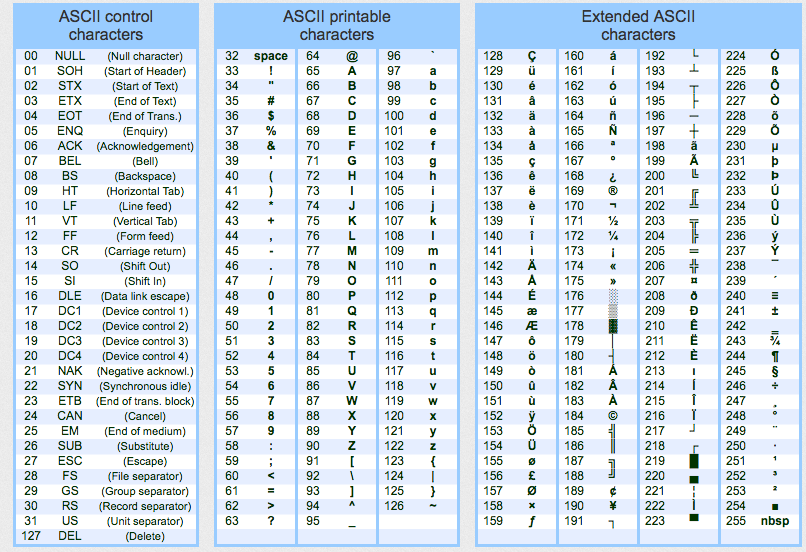
\includegraphics[width=11cm, keepaspectratio]{slike/Ascii_table-572996368.png}
                \caption{Tabla ASCII znakov}
                \caption*{\footnotesize Vir: \url{https://computersciencewiki.org/index.php/File:Ascii_table.png}}
                \label{fig:tabelaZnakov}
            \end{center}
        \end{figure}
    \subsection{Error correction}
        Odpravljanje napak (ang.: error correction) je skupek načeloma 
        matematičnih algoritmov s katerimi lažje opazimo in popravimo napake pri
        prenosu sporočila.
        Eden izmed prvih načinov prepoznave in odprave napak je Hammingov kod. 
        Najprej je potrebno razdeiti sporočilo na $
        \subsubsection{Cyclic redundancy check}

\newpage
\section{Empirični del – Digitalna vezja}
    \begin{figure}[h!]
        \begin{center}
            \caption{Moje prvo \LaTeX vezje}
            \begin{circuitikz} \draw
                (0, 2.5) to[american voltage source, l_=$U_{vh}$, i<=$I_{vh}$] (0, 0)
                (0, 2.5) to[D, l=$D_1$] (3.5, 2.5)
                to[R, l=$R_1$] (3.5, 0)
                to[short] (0, 0)
                ;
            \end{circuitikz}
            \label{fig:vezje1}
        \end{center}
    \end{figure}

\newpage

\begingroup
    \makeatletter
        \section{Viri in literatura}
            \nocite{*}
            \printbibliography[heading=none]
    \makeatother
\endgroup
\end{document}
